\documentclass{dlproblemset}
\usepackage{tikz}
\usetikzlibrary{positioning}
\tikzset{every picture/.style={line width=0.75pt}}

\title{Descida de Gradiente}
\subtitle{Lista de Exercícios}

\begin{document}

\begin{enumerate}[1)]

    \item Quando usamos a seguinte expressão $w_{(t+1)} = w_{(t)} - \eta \nabla \mathcal{L}$ para a atualização dos pesos de uma rede neural do tipo \textit{multilayer perceptron}, considerando que o gradiente está sendo estimado com base em uma única observação, temos qual variação do algoritmo de descida de gradiente?
    \begin{enumerate}[(a)]
	    \item \textit{Batch Gradient Descent}.
	    \item \textit{Mini Batch Gradient Descent}.
	    \item \textit{Stochastic Gradient Descent}.
	    \item \textit{Deterministic Gradient Descent}.
    \end{enumerate}
    %c

    \item Uma das modificações mais comuns no algoritmo de descida de gradiente envolve alterar a atualização dos pesos para que considere dois termos: um dos termos é o gradiente da função \textit{loss} em relação aos pesos considerando \textit{batch} atual; enquanto o segundo termo é um valor definido recursivamente que leva em consideração os gradientes anteriores. Essa modificação obedece a seguinte equação:

    \begin{align*}
        W_{(t+1)} &= W_{(t)} - \eta \mathcal{V}_{(t)} \\
        \mathcal{V}_{(t)} &= \beta \mathcal{V}_{(t-1)} + (1-\beta)\nabla \mathcal{L}
    \end{align*}
    \noindent Sendo que por definição $\mathcal{V}_{(0)} = 0$.

    Qual nome se dá para essa modificação na descida de gradiente?
    \begin{enumerate}[(a)]
        \item \textit{Batch Gradient Descent}
        \item \textit{Momentum}
        \item \textit{L2 Regularization}
        \item \textit{Stochastic Gradient Descent}
        \item \textit{Batch Normalization}
    \end{enumerate}
    %b

    \item O valor da função \textit{loss} da sua rede neural está oscilando ao invés de decrescer constantemente conforme esperado durante o treinamento. Supondo que você esteja utilizando \textit{Mini-Batch Gradient Descent}, quais das opções abaixo são boas modificações que você pode introduzir para tentar resolver esse problema?

	\begin{enumerate}[(a)]
	    \item Aparentemente isso é um problema dos dados, obter uma quantidade maior de dados para efetuar o treinamento é uma alternativa razoável.
	    \item Aumentar o valor hiperparâmetro \textit{learning rate} pode ajudar pois o processo de otimização vai chegar a um mínimo mais rápido.
	    \item Diminuir o valor do hiperparâmetro \textit{learning rate} pode ajudar pois passos menores evitam que o processo de otimização ``pule'' o mínimo em vez de assentar nele.
	    \item Aumentar o hiperparâmetro \textit{batch size} pode ajudar pois cada estimativa do gradiente passa a usar mais exemplos. Assim a variância da estimativa diminui e os passos da otimização ficam mais estáveis.
	\end{enumerate}
    %c, d

    \item Você está experimentando com diferentes \textit{learning rates} ao treinar uma rede neural específica. A evolução do valor da função \textit{loss} no decorrer das épocas usando \textit{learning rates} $0.1$ e $10^{-6}$ estão retratados na figura abaixo. Com base nesses resultados, qual seria um bom valor de \textit{learning rate} para testar a seguir?

    \begin{figure}[H]
        \centering
        \resizebox{0.55\linewidth}{!}{\input{problems/01-mlp/images/question_training_loss.tex}}
    \end{figure}

    \begin{enumerate}[(a)]
	    \item $0.2$
	    \item $10^{-4}$
	    \item $10^{-8}$
    \end{enumerate}
    %b

    \item Você se depara com uma situação na qual o seu time de pesquisa está usando o maior \textit{batch size} possível, respeitando apenas a limitação da memória disponível na GPU. Você entende existem argumentos a favor de um \textit{batch size} grande, contudo você quer trazer para a discussão argumentos contrários para incentivar o uso de \textit{batch sizes} menores. Dentre as alternativas abaixo, quais seriam bons argumentos para diminuir o \textit{batch size}?

    \begin{enumerate}[(a)]
        \item Um \textit{batch size} menor torna o processo de treino mais ruidoso, auxiliando na diminuição de \textit{overfitting}.
        \item Um \textit{batch size} menor pode tornar a paralelização mais otimizada e portanto o treinamento mais rápido.
        \item Um \textit{batch size} menor pode levar a uma maior generalização da rede, evitando mínimos locais.
        \item Um \textit{batch size} menor reduz o ruído no treinamento, melhorando a generalização do modelo treinado.
        \item O hiperparâmetro \textit{batch size} apenas diz respeito a limitações de \textit{hardware} e não influencia a solução que será otimizada.
    \end{enumerate}
    %a, c

    \item Dado que a descida de gradiente possui na sua formalização original a seguinte regra de atualização $\boldsymbol{\theta}_{t+1}=\boldsymbol{\theta}_t-\eta \nabla_{\boldsymbol{\theta}} J$. Por que a atualização dos pesos com $-\nabla_{\boldsymbol{\theta}} J$ diminui o valor da função de custo?

    \item Por que dizemos que a formulação original do \textit{momentum} calcula o gradiente ``no local errado''?

    \item Qual o efeito prático de normalizar o gradiente (conforme feito no Adam)?

    \item Qual a diferença de uma iteração para uma época?

    \item Considerando que $\boldsymbol{\theta}_t$ denota o vetor de parâmetros treináveis de uma rede neural na iteração $t$ e as seguintes informações:
    \begin{align*}
    \eta &= 0.1,\quad \beta=0.8, \quad \boldsymbol{\theta}_{0} =
      \begin{bmatrix}
        5 \\
        10
      \end{bmatrix},
      \quad \mathbf{v}_{0} =
      \begin{bmatrix}
        0 \\
        0
      \end{bmatrix},
    \\
    \nabla_{\boldsymbol{\theta}_{0}} J &=
      \begin{bmatrix}
        -2 \\
        5
      \end{bmatrix},
      \quad
      \nabla_{\boldsymbol{\theta}_{1}} J =
      \begin{bmatrix}
        -1 \\
        8
      \end{bmatrix},
      \quad
      \nabla_{\boldsymbol{\theta}_{2}} J =
      \begin{bmatrix}
        1 \\
        -1
      \end{bmatrix}
    \end{align*}
    \begin{enumerate}
        \item Como fica $\boldsymbol{\theta}_{1}$ ao seguir a regra de atualização do SGD?
        \item Como fica $\boldsymbol{\theta}_{1}$ ao seguir a regra de atualização da descida de gradiente com \textit{normalização}?
        \item Como fica $\boldsymbol{\theta}_{2}$ ao seguir a regra de atualização da descida de gradiente com \textit{momentum}?
        \item \emoji{skull-and-crossbones} Como fica $\boldsymbol{\theta}_{2}$ ao seguir a regra de atualização do otimizador \textsc{Adam}? (\textit{Nota}: ignore o $\beta = 0.8$ usado nos itens anteriores; aqui usamos os hiperparâmetros padrão do Adam, $\beta_1 = 0.9$ e $\beta_2 = 0.999$)
    \end{enumerate}

    \item Você treina o mesmo MLP quatro vezes, alterando apenas a taxa de aprendizado $\eta$ entre os treinos. As curvas A, B, C e D abaixo mostram a evolução da função de custo $\mathcal{L}$ ao longo das iterações em cada treino (todas partem da mesma inicialização). Assinale a alternativa que associa corretamente cada curva ao regime da taxa de aprendizado.

    \begin{center}
    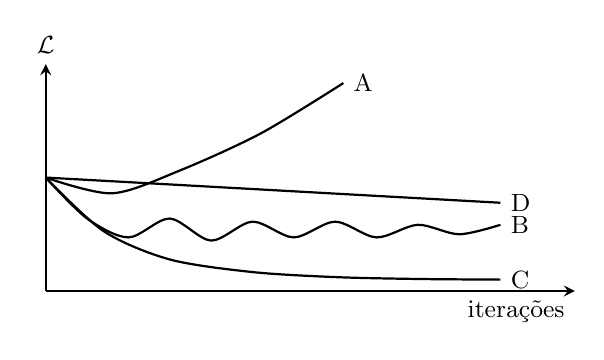
\begin{tikzpicture}[>=stealth, every node/.style={font=\small}, xscale=1.05, yscale=0.8]
        \draw[->] (0,0) -- (6.4,0) node[below left] {iterações};
        \draw[->] (0,0) -- (0,3.6) node[above] {$\mathcal{L}$};
        % A: diverges
        \draw[thick] plot[smooth] coordinates {(0,1.8) (0.8,1.55) (1.6,1.9) (2.6,2.5) (3.6,3.3)}
            node[right] {A};
        % B: fast drop then oscillates around plateau
        \draw[thick] plot[smooth] coordinates {(0,1.8) (0.5,1.15) (1.0,0.85) (1.5,1.15) (2.0,0.8) (2.5,1.1) (3.0,0.85) (3.5,1.1) (4.0,0.85) (4.5,1.05) (5.0,0.9) (5.5,1.05)}
            node[right] {B};
        % C: smooth convergence to low value
        \draw[thick] plot[smooth] coordinates {(0,1.8) (0.7,0.95) (1.5,0.5) (2.5,0.3) (3.5,0.22) (4.5,0.19) (5.5,0.18)}
            node[right] {C};
        % D: very slow, almost linear decline
        \draw[thick] plot[smooth] coordinates {(0,1.8) (1.1,1.72) (2.2,1.64) (3.3,1.56) (4.4,1.48) (5.5,1.4)}
            node[right] {D};
    \end{tikzpicture}
    \end{center}

    \begin{enumerate}[(a)]
        \item A: $\eta$ alta; \quad B: $\eta$ muito alta (divergência); \quad C: $\eta$ adequada; \quad D: $\eta$ muito baixa.
        \item A: $\eta$ muito alta (divergência); \quad B: $\eta$ adequada; \quad C: $\eta$ alta; \quad D: $\eta$ muito baixa.
        \item A: $\eta$ muito baixa; \quad B: $\eta$ alta; \quad C: $\eta$ adequada; \quad D: $\eta$ muito alta (divergência).
        \item A: $\eta$ muito alta (divergência); \quad B: $\eta$ alta; \quad C: $\eta$ muito baixa; \quad D: $\eta$ adequada.
        \item A: $\eta$ muito alta (divergência); \quad B: $\eta$ alta; \quad C: $\eta$ adequada; \quad D: $\eta$ muito baixa.
        \item A: $\eta$ alta; \quad B: $\eta$ muito baixa; \quad C: $\eta$ adequada; \quad D: $\eta$ muito alta (divergência).
        \item A: $\eta$ muito alta (divergência); \quad B: $\eta$ muito baixa; \quad C: $\eta$ alta; \quad D: $\eta$ adequada.
        \item A: $\eta$ adequada; \quad B: $\eta$ alta; \quad C: $\eta$ muito alta (divergência); \quad D: $\eta$ muito baixa.
    \end{enumerate}
    %e

    \item Um único parâmetro $\theta$ é otimizado por descida de gradiente com \textit{momentum}, na formulação vista em aula:
    \[
    v_{t+1} = \beta\,v_{t} + (1-\beta)\,\nabla_{\theta}\mathcal{L}(\theta_{t}), \qquad \theta_{t+1} = \theta_{t} - \eta\,v_{t+1},
    \]
    com $\eta = 0{,}1$, $\beta = 0{,}5$, $v_0 = 0$ e $\theta_0 = 1$. Os gradientes observados nas duas primeiras iterações são $\nabla_{\theta}\mathcal{L}(\theta_0) = 4$ e $\nabla_{\theta}\mathcal{L}(\theta_1) = 2$. Qual o valor de $\theta_2$ após \textbf{duas} atualizações?
    \begin{enumerate}[(a)]
        \item $0{,}2$
        \item $0{,}4$
        \item $0{,}5$
        \item $0{,}6$
        \item $0{,}7$
        \item $0{,}8$
        \item $1{,}0$
        \item $1{,}4$
    \end{enumerate}
    %d

    \item Um único parâmetro $\theta$ é otimizado com Adam (hiperparâmetros $\beta_1 = 0.9$, $\beta_2 = 0.999$, $\eta = 0.01$, $\epsilon \approx 10^{-8}$). Os acumuladores começam zerados ($m_0 = v_0 = 0$). Na primeira iteração ($t = 1$) o gradiente é $g_1 = 3$. Lembrando que Adam aplica correção de viés $\hat{m} = m / (1 - \beta_1^{t})$ e $\hat{v} = v / (1 - \beta_2^{t})$ e atualiza $\theta \leftarrow \theta - \eta\,\hat{m}/(\sqrt{\hat{v}} + \epsilon)$, qual é, aproximadamente, o módulo da atualização $|\Delta\theta| = |\theta_1 - \theta_0|$ neste primeiro passo?
    \begin{enumerate}[(a)]
        \item $0.0316$
        \item $0.03$
        \item $0.01$
        \item $0.003$
        \item $0.1$
        \item $0.3$
        \item $0.0001$
        \item $1.0$
    \end{enumerate}
    %c

    \item Avalie as cinco afirmações a seguir sobre otimização em MLPs:

    \textbf{I.} Na descida de gradiente em lote (\textit{batch GD}), cada iteração usa o gradiente médio sobre \emph{todo} o conjunto de treinamento; já no SGD, cada iteração usa o gradiente de uma \emph{única} instância.

    \textbf{II.} O momentum acumula uma média móvel exponencial dos gradientes; com $\beta = 0$, a atualização reduz-se à descida de gradiente padrão.

    \textbf{III.} No AdaGrad, o acumulador de gradientes ao quadrado cresce monotonicamente, de modo que a taxa de aprendizado efetiva por parâmetro tende a diminuir ao longo do treinamento.

    \textbf{IV.} O momentum de Nesterov avalia o gradiente na posição atual $\theta_t$.

    \textbf{V.} Em Adam, a correção de viés ($\hat{m}_t = m_t/(1-\beta_1^{t})$ e $\hat{v}_t = v_t/(1-\beta_2^{t})$) torna-se progressivamente mais relevante à medida que $t$ cresce, pois os denominadores $1-\beta_1^{t}$ e $1-\beta_2^{t}$ se afastam cada vez mais de $1$.

    \begin{enumerate}[(a)]
        \item Apenas I, III e V estão corretas.
        \item Apenas I, II, III e IV estão corretas.
        \item Apenas II, III e IV estão corretas.
        \item Apenas I e III estão corretas.
        \item Apenas I, II e III estão corretas.
        \item Apenas I, II e V estão corretas.
        \item Todas as afirmações estão corretas.
        \item Apenas III e V estão corretas.
    \end{enumerate}
    %e

    \item A aproximação de primeira ordem da série de Taylor prevê que, ao aplicar a atualização $\boldsymbol{\theta}_{t+1} = \boldsymbol{\theta}_t - \eta\,\nabla_{\boldsymbol{\theta}}\mathcal{L}$, a variação da loss é $\Delta\mathcal{L} \approx -\eta\,\|\nabla_{\boldsymbol{\theta}}\mathcal{L}\|^2$. Considere $\mathcal{L}(\theta_1, \theta_2) = \theta_1^2 + 2\theta_2^2$, o ponto $\boldsymbol{\theta}_t = (2;\ 1)$ e a taxa de aprendizado $\eta = 0{,}1$. Quais são, respectivamente, a variação \emph{prevista} pela aproximação linear e a variação \emph{real} da loss após um passo?

    \begin{enumerate}[(a)]
        \item Prevista $-3{,}20$ e real $-2{,}72$.
        \item Prevista $-2{,}72$ e real $-3{,}20$.
        \item Prevista $-3{,}20$ e real $-3{,}20$.
        \item Prevista $-0{,}32$ e real $-2{,}72$.
        \item Prevista $-3{,}20$ e real $-3{,}08$.
        \item Prevista $-2{,}00$ e real $-2{,}16$.
        \item Prevista $-3{,}20$ e real $-3{,}68$.
        \item Prevista $-6{,}40$ e real $-2{,}72$.
    \end{enumerate}
    %a

    \item Em um modelo com apenas dois parâmetros treináveis, o gradiente no ponto atual é $\nabla_{\boldsymbol{\theta}}\mathcal{L} = (2;\ 2)$. Considere os cinco candidatos a direção de atualização $\Delta\boldsymbol{\theta}$ abaixo, todos aplicados com a mesma taxa de aprendizado $\eta > 0$ pequena:
    \[
    \mathbf{v}_1 = (-2;\ -2), \qquad
    \mathbf{v}_2 = (-3;\ 1), \qquad
    \mathbf{v}_3 = (2;\ -2), \qquad
    \mathbf{v}_4 = (3;\ 1), \qquad
    \mathbf{v}_5 = (-1;\ 3).
    \]
    Quais desses candidatos reduzem o valor da loss segundo a aproximação de primeira ordem?

    \begin{enumerate}[(a)]
        \item Apenas $\mathbf{v}_1$.
        \item Apenas $\mathbf{v}_1$ e $\mathbf{v}_3$.
        \item Apenas $\mathbf{v}_2$ e $\mathbf{v}_5$.
        \item Apenas $\mathbf{v}_1$, $\mathbf{v}_2$ e $\mathbf{v}_3$.
        \item Apenas $\mathbf{v}_1$, $\mathbf{v}_2$ e $\mathbf{v}_5$.
        \item Apenas $\mathbf{v}_1$ e $\mathbf{v}_2$.
        \item Apenas $\mathbf{v}_3$ e $\mathbf{v}_4$.
        \item $\mathbf{v}_1$, $\mathbf{v}_2$, $\mathbf{v}_3$ e $\mathbf{v}_5$.
    \end{enumerate}
    %f

    \item Compare dois otimizadores na \textbf{primeira} iteração ($t = 0$, com $\mathbf{m}_0 = \mathbf{v}_0 = \mathbf{0}$ e $\epsilon \approx 0$). Ambos acumulam as mesmas médias móveis,
    \[
    \mathbf{m}_{1} = \beta_1\,\mathbf{m}_{0} + (1 - \beta_1)\,\nabla_{\boldsymbol{\theta}}\mathcal{L}, \qquad
    \mathbf{v}_{1} = \beta_2\,\mathbf{v}_{0} + (1 - \beta_2)\,\bigl(\nabla_{\boldsymbol{\theta}}\mathcal{L}\bigr)^{2} ,
    \]
    mas o primeiro atualiza com $\boldsymbol{\theta}_{1} = \boldsymbol{\theta}_{0} - \eta\,\mathbf{m}_{1} / (\sqrt{\mathbf{v}_{1}} + \epsilon)$, sem correção de viés, enquanto o Adam aplica a correção antes de dividir. Com $\eta = 0{,}1$, $\beta_1 = \beta_2 = 0{,}99$, $\boldsymbol{\theta}_0 = (4;\ -2)$ e $\nabla_{\boldsymbol{\theta}}\mathcal{L}(\boldsymbol{\theta}_0) = (2;\ -4)$, quais são os dois valores de $\boldsymbol{\theta}_1$?
    \begin{enumerate}[(a)]
        \item Sem correção $(3{,}90;\ -1{,}90)$ e Adam $(3{,}99;\ -1{,}99)$.
        \item Sem correção $(3{,}80;\ -1{,}60)$ e Adam $(3{,}90;\ -1{,}90)$.
        \item Sem correção $(3{,}99;\ -1{,}99)$ e Adam $(3{,}90;\ -1{,}90)$.
        \item Sem correção $(3{,}99;\ -1{,}99)$ e Adam $(3{,}00;\ -1{,}00)$.
        \item Sem correção $(3{,}90;\ -1{,}90)$ e Adam $(3{,}90;\ -1{,}90)$.
        \item Sem correção $(3{,}99;\ -1{,}99)$ e Adam $(3{,}99;\ -1{,}99)$.
        \item Sem correção $(3{,}99;\ -1{,}99)$ e Adam $(3{,}80;\ -1{,}60)$.
        \item Sem correção $(3{,}00;\ -1{,}00)$ e Adam $(3{,}90;\ -1{,}90)$.
    \end{enumerate}
    %c

    \item Associe cada otimizador (coluna da esquerda) ao comportamento observado durante o treinamento (coluna da direita).

    \begin{center}
    \begin{tabular}{p{0.22\linewidth} p{0.70\linewidth}}
    \textbf{1.} \textit{Momentum} & \textbf{(i)} a taxa efetiva de cada parâmetro volta a crescer quando os gradientes recentes desse parâmetro ficam pequenos. \\
    \textbf{2.} Nesterov & \textbf{(ii)} em um vale estreito, as oscilações transversais se cancelam e o avanço ao longo do vale acelera. \\
    \textbf{3.} AdaGrad & \textbf{(iii)} a taxa efetiva de cada parâmetro só diminui, e após muitas iterações o treinamento praticamente estaciona. \\
    \textbf{4.} RMSProp & \textbf{(iv)} o gradiente é avaliado no ponto para onde a memória levaria, e o passo é corrigido antes de uma curva do vale. \\
    \end{tabular}
    \end{center}

    \begin{enumerate}[(a)]
        \item 1-(iv); 2-(ii); 3-(iii); 4-(i)
        \item 1-(iii); 2-(i); 3-(ii); 4-(iv)
        \item 1-(ii); 2-(iv); 3-(i); 4-(iii)
        \item 1-(i); 2-(iii); 3-(ii); 4-(iv)
        \item 1-(iv); 2-(ii); 3-(i); 4-(iii)
        \item 1-(iii); 2-(i); 3-(iv); 4-(ii)
        \item 1-(i); 2-(iii); 3-(iv); 4-(ii)
        \item 1-(ii); 2-(iv); 3-(iii); 4-(i)
    \end{enumerate}
    %h

    \item Uma rede é treinada com dois objetivos, representados pelas funções de custo $\mathcal{L}_1$ e $\mathcal{L}_2$. No ponto atual dos parâmetros, os gradientes são os mostrados abaixo.

    \begin{center}
    \begin{minipage}{0.3\linewidth}
    \[
    \nabla_{\boldsymbol{\theta}}\mathcal{L}_1 = \begin{bmatrix} 4 \\ 1 \end{bmatrix}
    \]
    \[
    \nabla_{\boldsymbol{\theta}}\mathcal{L}_2 = \begin{bmatrix} -2 \\ 1 \end{bmatrix}
    \]
    \end{minipage}%
    \begin{minipage}{0.68\linewidth}\centering
    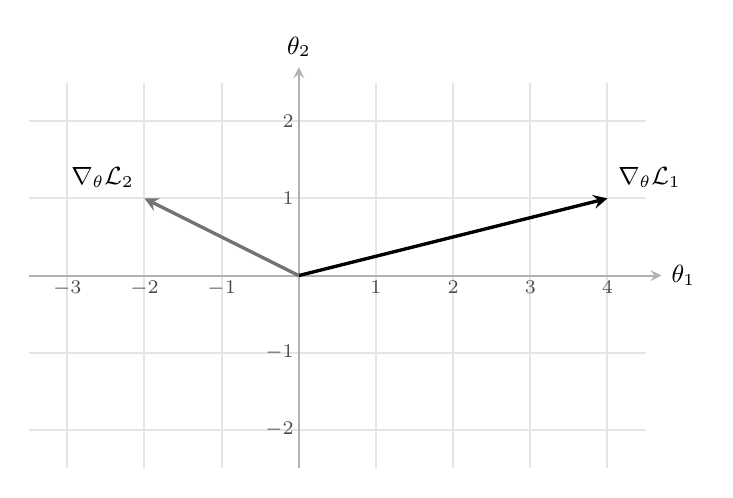
\begin{tikzpicture}[scale=0.98, >=stealth]
      \foreach \g in {-3,-2,-1,1,2,3,4} { \draw[gray!20] (\g,-2.5) -- (\g,2.5); }
      \foreach \g in {-2,-1,1,2} { \draw[gray!20] (-3.5,\g) -- (4.5,\g); }
      \draw[gray!60, ->] (-3.5,0) -- (4.7,0) node[right, font=\small, black] {$\theta_1$};
      \draw[gray!60, ->] (0,-2.5) -- (0,2.7) node[above, font=\small, black] {$\theta_2$};
      \foreach \t in {-3,-2,-1,1,2,3,4} \node[font=\scriptsize, below, gray!60!black, inner sep=1.5pt] at (\t,0) {$\t$};
      \foreach \t in {-2,-1,1,2} \node[font=\scriptsize, left, gray!60!black, inner sep=1.5pt] at (0,\t) {$\t$};
      \draw[->, very thick] (0,0) -- (4,1) node[above right, font=\small] {$\nabla_{\boldsymbol{\theta}}\mathcal{L}_1$};
      \draw[->, very thick, black!55] (0,0) -- (-2,1) node[above left, font=\small, black] {$\nabla_{\boldsymbol{\theta}}\mathcal{L}_2$};
    \end{tikzpicture}
    \end{minipage}
    \end{center}

    Você percebe que o passo usual do SGD sobre $\mathcal{L}_1$ melhora o objetivo 1, mas degrada o objetivo 2.

    Considere atualizações da forma $\boldsymbol{\theta}_{t+1} = \boldsymbol{\theta}_t + \eta\,\Delta\boldsymbol{\theta}$, com $\eta > 0$ pequeno. Pela aproximação de primeira ordem, a variação de cada função de custo é
    \[
    \mathcal{L}_k(\boldsymbol{\theta}_t + \eta\,\Delta\boldsymbol{\theta}) - \mathcal{L}_k(\boldsymbol{\theta}_t)
    \approx \eta\,\Delta\boldsymbol{\theta}^{\top}\nabla_{\boldsymbol{\theta}}\mathcal{L}_k
    = \eta\,\|\Delta\boldsymbol{\theta}\|\,\|\nabla_{\boldsymbol{\theta}}\mathcal{L}_k\|\cos(\alpha_k),
    \]
    em que $\alpha_k$ é o ângulo entre $\Delta\boldsymbol{\theta}$ e $\nabla_{\boldsymbol{\theta}}\mathcal{L}_k$. Qual direção $\Delta\boldsymbol{\theta}$ reduz $\mathcal{L}_1$ e mantém $\mathcal{L}_2$ inalterada segundo essa aproximação?

    \begin{enumerate}[(a)]
        \item $\Delta\boldsymbol{\theta} = \bigl[\,-4 \quad -1\,\bigr]^{\top}$
        \item $\Delta\boldsymbol{\theta} = \bigl[\,-1 \quad -1\,\bigr]^{\top}$
        \item $\Delta\boldsymbol{\theta} = \bigl[\,-2 \quad -2\,\bigr]^{\top}$
        \item $\Delta\boldsymbol{\theta} = \bigl[\,-1 \quad -2\,\bigr]^{\top}$
        \item $\Delta\boldsymbol{\theta} = \bigl[\,-2 \quad 1\,\bigr]^{\top}$
        \item $\Delta\boldsymbol{\theta} = \bigl[\,1 \quad 2\,\bigr]^{\top}$
        \item $\Delta\boldsymbol{\theta} = \bigl[\,1 \quad -4\,\bigr]^{\top}$
        \item $\Delta\boldsymbol{\theta} = \bigl[\,-6 \quad 0\,\bigr]^{\top}$
    \end{enumerate}
    %d

    \item Em uma camada com matriz de pesos $\mathbf{W}$ de formato $2 \times 2$, o \textit{momentum} acumulado nesta iteração e a sua SVD, $\mathbf{M}_{t+1} = \mathbf{U}\boldsymbol{\Sigma}\mathbf{V}^{\top}$, são
    \[
    \mathbf{M}_{t+1} = \begin{bmatrix} 12 & 4 \\ 11 & 12 \end{bmatrix}, \qquad
    \mathbf{U} = \frac{1}{5}\begin{bmatrix} 3 & -4 \\ 4 & 3 \end{bmatrix}, \qquad
    \boldsymbol{\Sigma} = \begin{bmatrix} 20 & 0 \\ 0 & 5 \end{bmatrix}, \qquad
    \mathbf{V} = \frac{1}{5}\begin{bmatrix} 4 & -3 \\ 3 & 4 \end{bmatrix}.
    \]
    Os dois otimizadores atualizam a camada como $\mathbf{W}_{t+1} = \mathbf{W}_t - \eta\,\mathbf{D}$, cada um com a sua matriz de direção $\mathbf{D}$. Suponha que o Adam tenha histórico de gradientes estável, com $\widetilde{\mathbf{m}}_{t+1} = \mathbf{M}_{t+1}$ e $\widetilde{\mathbf{v}}_{t+1} = \widetilde{\mathbf{m}}_{t+1}^{2}$ (entrada a entrada, $\epsilon \approx 0$), e que o Muon receba o mesmo $\mathbf{M}_{t+1}$. Quais são $\mathbf{D}_{\text{Adam}}$ e $\mathbf{D}_{\text{Muon}}$?

    \begin{enumerate}[(a)]
        \item $\mathbf{D}_{\text{Adam}} = \begin{bmatrix} 1 & 1 \\ 1 & 1 \end{bmatrix}$, \quad $\mathbf{D}_{\text{Muon}} = \begin{bmatrix} 0{,}96 & 0{,}28 \\ -0{,}28 & 0{,}96 \end{bmatrix}$
        \item $\mathbf{D}_{\text{Adam}} = \begin{bmatrix} 0{,}96 & -0{,}28 \\ 0{,}28 & 0{,}96 \end{bmatrix}$, \quad $\mathbf{D}_{\text{Muon}} = \begin{bmatrix} 0{,}96 & -0{,}28 \\ 0{,}28 & 0{,}96 \end{bmatrix}$
        \item $\mathbf{D}_{\text{Adam}} = \begin{bmatrix} 1 & 1 \\ 1 & 1 \end{bmatrix}$, \quad $\mathbf{D}_{\text{Muon}} = \begin{bmatrix} 1 & 1 \\ 1 & 1 \end{bmatrix}$
        \item $\mathbf{D}_{\text{Adam}} = \begin{bmatrix} 0{,}96 & -0{,}28 \\ 0{,}28 & 0{,}96 \end{bmatrix}$, \quad $\mathbf{D}_{\text{Muon}} = \begin{bmatrix} 0{,}6 & 0{,}2 \\ 0{,}55 & 0{,}6 \end{bmatrix}$
        \item $\mathbf{D}_{\text{Adam}} = \begin{bmatrix} 0{,}96 & -0{,}28 \\ 0{,}28 & 0{,}96 \end{bmatrix}$, \quad $\mathbf{D}_{\text{Muon}} = \begin{bmatrix} 0{,}96 & 0{,}28 \\ -0{,}28 & 0{,}96 \end{bmatrix}$
        \item $\mathbf{D}_{\text{Adam}} = \begin{bmatrix} 1 & 1 \\ 1 & 1 \end{bmatrix}$, \quad $\mathbf{D}_{\text{Muon}} = \begin{bmatrix} 0{,}96 & -0{,}28 \\ 0{,}28 & 0{,}96 \end{bmatrix}$
        \item $\mathbf{D}_{\text{Adam}} = \begin{bmatrix} 1 & 1 \\ 1 & 1 \end{bmatrix}$, \quad $\mathbf{D}_{\text{Muon}} = \begin{bmatrix} 0{,}6 & 0{,}2 \\ 0{,}55 & 0{,}6 \end{bmatrix}$
        \item $\mathbf{D}_{\text{Adam}} = \begin{bmatrix} 0{,}96 & -0{,}28 \\ 0{,}28 & 0{,}96 \end{bmatrix}$, \quad $\mathbf{D}_{\text{Muon}} = \begin{bmatrix} 1 & 1 \\ 1 & 1 \end{bmatrix}$
    \end{enumerate}
    %f

\end{enumerate}

\newpage

\subsection*{Gabarito}
\color{blue}
\begin{enumerate}[1)]

    \item c. Estimar o gradiente com uma única observação caracteriza o \textit{Stochastic Gradient Descent}. O \textit{Batch Gradient Descent} usa o conjunto de treino inteiro em cada passo e o \textit{Mini Batch} usa subconjuntos com mais de uma observação; \textit{Deterministic Gradient Descent} não é uma variação padrão do algoritmo.

    \item b. A equação define uma média móvel exponencial dos gradientes: $\mathcal{V}_t$ acumula o histórico com peso $\beta$ e o gradiente atual com peso $1-\beta$, que é exatamente o \textit{momentum}. Não há termo de penalidade sobre os pesos (L2) nem normalização de ativações (\textit{batch normalization}) na expressão.

    \item c, d. A oscilação indica passos grandes ou ruidosos demais. Diminuir a taxa de aprendizado reduz o tamanho do passo e permite assentar no vale (c), e aumentar o \textit{batch size} coloca mais exemplos em cada estimativa do gradiente, tornando os passos mais estáveis (d). Obter mais dados (a) não muda a dinâmica do passo, e aumentar a taxa de aprendizado (b) agrava a oscilação.

    \item b. Com $0.1$ a \textit{loss} cai rápido mas se comporta de forma instável (taxa alta demais) e com $10^{-6}$ o decaimento é lento demais. O próximo palpite razoável fica entre os dois extremos em escala logarítmica, como $10^{-4}$. Testar $0.2$ (a) aumentaria a instabilidade e $10^{-8}$ (c) seria ainda mais lento que o caso já inviável.

    \item a, c. O ruído da estimativa do gradiente com \textit{batches} menores atua como regularização implícita, dificultando a memorização do conjunto de treino (a) e ajudando a escapar de mínimos ruins (c). A alternativa (b) é falsa pois \textit{batches} menores aproveitam pior o paralelismo da GPU, (d) afirma o oposto de (a) e (e) ignora o efeito do \textit{batch size} na solução encontrada.

    \item O gradiente aponta na direção de maior crescimento local da função de custo, então atualizar os pesos na direção contrária diminui o custo. Formalmente, pela expansão de primeira ordem, $J(\boldsymbol{\theta} - \eta\nabla_{\boldsymbol{\theta}} J) \approx J(\boldsymbol{\theta}) - \eta\,\|\nabla_{\boldsymbol{\theta}} J\|^2$, e como $\|\nabla_{\boldsymbol{\theta}} J\|^2 \geq 0$, um passo suficientemente pequeno na direção $-\nabla_{\boldsymbol{\theta}} J$ reduz o valor de $J$.

    \item Dizemos que o gradiente está atrasado pois, devido ao \textit{momentum}, já existe uma atualização dos pesos conforme o histórico dos gradientes. Essa observação leva a definição do \textit{Nesterov Accelerated Momentum}: como a atualização vai deslocar os pesos pelo termo de histórico $\beta v_t$ de qualquer forma, é mais informativo avaliar o gradiente no ponto para onde os pesos estão indo (o ponto \textit{lookahead}) do que no ponto atual, e o Nesterov faz exatamente essa correção.

    \item Ao normalizar o gradiente, fica mais fácil definir uma taxa de aprendizado que funcione igualmente bem para todos os parâmetros da rede. Sem normalização, parâmetros com gradientes de escalas muito diferentes exigiriam taxas de aprendizado diferentes; ao dividir cada componente pela raiz do segundo momento acumulado, o passo efetivo de cada parâmetro fica com magnitude comparável, próxima de $\eta$.

    \item Uma iteração consiste na apresentação de algumas instâncias para o modelo, sob as quais são realizados \textit{Forward Pass}, cálculo da função de custo, \textit{Backward Pass} e otimização. Uma época ocorre quando foram feitas iterações suficientes para ver todas as instâncias do conjunto de treinamento 1 vez.

    \item
    \begin{align*}
    \eta &= 0.1, \quad \boldsymbol{\theta}_{0} =
      \begin{bmatrix}
        5 \\
        10
      \end{bmatrix},
      \quad \mathbf{v}_{0} =
      \begin{bmatrix}
        0 \\
        0
      \end{bmatrix},
    \\
    \nabla_{\boldsymbol{\theta}_{0}} J &=
      \begin{bmatrix}
        -2 \\
        5
      \end{bmatrix},
      \quad
      \nabla_{\boldsymbol{\theta}_{1}} J =
      \begin{bmatrix}
        -1 \\
        8
      \end{bmatrix},
      \quad
      \nabla_{\boldsymbol{\theta}_{2}} J =
      \begin{bmatrix}
        1 \\
        -1
      \end{bmatrix}
    \end{align*}
    \begin{enumerate}
        \item
        \begin{align*}
            \boldsymbol{\theta}_{1} =
      \begin{bmatrix}
        5 \\
        10
      \end{bmatrix} -0.1\begin{bmatrix}
        -2 \\
        5
      \end{bmatrix} = \begin{bmatrix}
        5.2 \\
        9.5
      \end{bmatrix}
        \end{align*}

        \item
                \begin{align*}
            \boldsymbol{\theta}_{1} =
      \begin{bmatrix}
        5 \\
        10
      \end{bmatrix} -0.1\left (\begin{bmatrix}
        -2 \\
        5
      \end{bmatrix}\div\begin{bmatrix}
        2 \\
        5
      \end{bmatrix}\right) = \begin{bmatrix}
        5.1 \\
        9.9
      \end{bmatrix}
        \end{align*}
        \item

\begin{align*}
            \mathbf{v}_1=0.8\begin{bmatrix}
        0 \\
        0
      \end{bmatrix} + (1-0.8)\begin{bmatrix}
        -2 \\
        5
      \end{bmatrix}=\begin{bmatrix}
        -0.4 \\
        1
      \end{bmatrix}\\
      \boldsymbol{\theta}_{1} =
      \begin{bmatrix}
        5 \\
        10
      \end{bmatrix} -0.1\begin{bmatrix}
        -0.4 \\
        1
      \end{bmatrix} = \begin{bmatrix}
        5.04 \\
        9.9
      \end{bmatrix}\\
      \mathbf{v}_2=0.8\begin{bmatrix}
        -0.4 \\
        1
      \end{bmatrix} + (1-0.8)\begin{bmatrix}
        -1 \\
        8
      \end{bmatrix}=\begin{bmatrix}
        -0.52 \\
        2.40
      \end{bmatrix}\\
      \boldsymbol{\theta}_{2} =
      \begin{bmatrix}
        5.04 \\
        9.9
      \end{bmatrix} -0.1\begin{bmatrix}
        -0.52 \\
        2.40
      \end{bmatrix} = \begin{bmatrix}
        5.092 \\
        9.660
      \end{bmatrix}
        \end{align*}

        \item \emoji{skull-and-crossbones}
        Considerando as regras de atualização do \textsc{Adam} com $\eta = 0.1$, $\beta = 0.9$ e $\gamma = 0.999$, podemos calcular o valor de $\boldsymbol{\theta}_{2}$.

Primeiro, calculamos $\boldsymbol{\theta}_{1}$ para a iteração $t=1$:

  Momento ($\mathbf{m}_1$):
    $$\mathbf{m}_{1} = \beta \mathbf{m}_{0} + (1-\beta )\nabla_{\boldsymbol{\theta}_{0}}J = 0.9\begin{bmatrix} 0\\ 0 \end{bmatrix} + (1-0.9)\begin{bmatrix} -2\\ 5 \end{bmatrix} = \begin{bmatrix} 0\\ 0 \end{bmatrix} + 0.1\begin{bmatrix} -2\\ 5 \end{bmatrix} = \begin{bmatrix} -0.2\\ 0.5 \end{bmatrix}$$

  Termo normalizador ($\mathbf{v}_1$):
    $$\mathbf{v}_{1} = \gamma \mathbf{v}_{0} + (1-\gamma )(\nabla_{\boldsymbol{\theta}_{0}}J)^2 = 0.999\begin{bmatrix} 0\\ 0 \end{bmatrix} + (1-0.999)\begin{bmatrix} (-2)^2\\ 5^2 \end{bmatrix} = \begin{bmatrix} 0\\ 0 \end{bmatrix} + 0.001\begin{bmatrix} 4\\ 25 \end{bmatrix} = \begin{bmatrix} 0.004\\ 0.025 \end{bmatrix}$$

  Correção de viés (\textit{bias correction}):
    $$\hat{\mathbf{m}}_{1} = \frac{\mathbf{m}_{1}}{1 - \beta ^{1}} = \frac{\begin{bmatrix} -0.2\\ 0.5 \end{bmatrix}}{1 - 0.9} = \begin{bmatrix} -2\\ 5 \end{bmatrix}$$   $$\hat{\mathbf{v}}_{1} = \frac{\mathbf{v}_{1}}{1 - \gamma ^{1}} = \frac{\begin{bmatrix} 0.004\\ 0.025 \end{bmatrix}}{1 - 0.999} = \begin{bmatrix} 4\\ 25 \end{bmatrix}$$

  Atualização de $\boldsymbol{\theta}_1$:
    $$\boldsymbol{\theta}_{1} = \boldsymbol{\theta}_{0} - \eta \frac{\hat{\mathbf{m}}_{1}}{\sqrt{\hat{\mathbf{v}}_{1}} + \epsilon} = \begin{bmatrix} 5\\ 10 \end{bmatrix} - 0.1\begin{bmatrix} \frac{-2}{\sqrt{4}}\\ \frac{5}{\sqrt{25}} \end{bmatrix} = \begin{bmatrix} 5\\ 10 \end{bmatrix} - 0.1\begin{bmatrix} -1\\ 1 \end{bmatrix} = \begin{bmatrix} 5.1\\ 9.9 \end{bmatrix}$$

Agora, calculamos $\boldsymbol{\theta}_{2}$ para a iteração $t=2$:

  Momento ($\mathbf{m}_2$):
    $$\mathbf{m}_{2} = \beta \mathbf{m}_{1} + (1-\beta )\nabla_{\boldsymbol{\theta}_{1}}J = 0.9\begin{bmatrix} -0.2\\ 0.5 \end{bmatrix} + (1-0.9)\begin{bmatrix} -1\\ 8 \end{bmatrix} = \begin{bmatrix} -0.18\\ 0.45 \end{bmatrix} + 0.1\begin{bmatrix} -1\\ 8 \end{bmatrix} = \begin{bmatrix} -0.28\\ 1.25 \end{bmatrix}$$

  Termo normalizador ($\mathbf{v}_2$):
    $$\begin{aligned}\mathbf{v}_{2} &= \gamma \mathbf{v}_{1} + (1-\gamma )(\nabla_{\boldsymbol{\theta}_{1}}J)^2 = 0.999\begin{bmatrix} 0.004\\ 0.025 \end{bmatrix} + (1-0.999)\begin{bmatrix} (-1)^2\\ 8^2 \end{bmatrix} \\ &= \begin{bmatrix} 0.003996\\ 0.024975 \end{bmatrix} + 0.001\begin{bmatrix} 1\\ 64 \end{bmatrix} = \begin{bmatrix} 0.004996\\ 0.088975 \end{bmatrix}\end{aligned}$$

  Correção de viés (\textit{bias correction}):
    $$\hat{\mathbf{m}}_{2} = \frac{\mathbf{m}_{2}}{1 - \beta ^{2}} = \frac{\begin{bmatrix} -0.28\\ 1.25 \end{bmatrix}}{1 - 0.9^2} = \frac{\begin{bmatrix} -0.28\\ 1.25 \end{bmatrix}}{0.19} \approx \begin{bmatrix} -1.47368\\ 6.57895 \end{bmatrix}$$   $$\hat{\mathbf{v}}_{2} = \frac{\mathbf{v}_{2}}{1 - \gamma ^{2}} = \frac{\begin{bmatrix} 0.004996\\ 0.088975 \end{bmatrix}}{1 - 0.999^2} = \frac{\begin{bmatrix} 0.004996\\ 0.088975 \end{bmatrix}}{0.001999} \approx \begin{bmatrix} 2.49925\\ 44.50975 \end{bmatrix}$$

  Atualização de $\boldsymbol{\theta}_2$:
    $$\boldsymbol{\theta}_{2} = \boldsymbol{\theta}_{1} - \eta \frac{\hat{\mathbf{m}}_{2}}{\sqrt{\hat{\mathbf{v}}_{2}} + \epsilon} = \begin{bmatrix} 5.1\\ 9.9 \end{bmatrix} - 0.1\begin{bmatrix} \frac{-1.47368}{\sqrt{2.49925}}\\ \frac{6.57895}{\sqrt{44.50975}} \end{bmatrix} \approx \begin{bmatrix} 5.1\\ 9.9 \end{bmatrix} - 0.1\begin{bmatrix} -0.9322\\ 0.9861 \end{bmatrix} = \begin{bmatrix} 5.1932\\ 9.8014 \end{bmatrix}$$

Portanto, o valor de $\boldsymbol{\theta}_{2}$ ao seguir a regra de atualização do \textsc{Adam} é:
$$\boldsymbol{\theta}_{2} \approx \begin{bmatrix} 5.193\\ 9.801 \end{bmatrix}$$
    \end{enumerate}

    \item e. Leitura das curvas: \textbf{A} sobe após uma queda inicial, ou seja, o custo diverge, comportamento típico de $\eta$ muito alta. \textbf{B} cai rápido mas passa a oscilar em torno de um patamar acima do mínimo: os passos são grandes demais para entrar no vale, $\eta$ alta. \textbf{C} decai de forma suave e estabiliza em valor baixo: $\eta$ adequada. \textbf{D} decai quase linearmente e muito devagar: $\eta$ muito baixa. Os erros embutidos nas demais alternativas se agrupam em três confusões: tratar a oscilação de B como se fosse convergência ($\eta$ adequada), ou como divergência (alternativas (a), (b) e (h)); tratar o declínio lento e constante de D como se fosse o regime adequado, quando na prática o treino não converge em tempo útil (alternativas (d) e (g)); e inverter divergência com lentidão, associando a curva ascendente A a $\eta$ pequena (alternativas (c) e (f)). Os sinais de cada regime são: divergência = custo crescente; $\eta$ alta = oscilação em patamar; adequada = queda suave até valor baixo; muito baixa = queda lenta quase linear.

    \item d. Primeira iteração: $v_1 = 0{,}5 \cdot 0 + 0{,}5 \cdot 4 = 2$ e $\theta_1 = 1 - 0{,}1 \cdot 2 = 0{,}8$. Segunda iteração: $v_2 = 0{,}5 \cdot 2 + 0{,}5 \cdot 2 = 2$ e $\theta_2 = 0{,}8 - 0{,}1 \cdot 2 = 0{,}6$. A alternativa (a) $0{,}2$ resulta de omitir o fator $(1-\beta)$ (convenção Polyak/PyTorch, $v_{t+1} = \beta v_t + \nabla\mathcal{L}$), que não é a formulação dada no enunciado; (b) $0{,}4$ é o resultado de SGD puro, ignorando o acumulador de \textit{momentum}; (c) $0{,}5$ resulta de aplicar $(1-\beta)$ apenas na primeira iteração ($v_2 = 0{,}5\cdot 2 + 2 = 3$); (e) $0{,}7$ corresponde a um único passo com o gradiente médio ($\theta = 1 - 0{,}1 \cdot 3$); (f) $0{,}8$ é o valor de $\theta_1$, apenas uma iteração; (g) $1{,}0$ assume que o \textit{momentum} se anula e $\theta$ volta ao valor inicial, o que não ocorre, pois os gradientes têm o mesmo sinal; (h) $1{,}4$ resulta de somar em vez de subtrair as atualizações (subida de gradiente).

    \item c. Com $m_0 = v_0 = 0$ e $g_1 = 3$: $m_1 = 0.1\cdot 3 = 0.3$ e $v_1 = 0.001\cdot 3^2 = 0.009$. Correção de viés em $t = 1$: $\hat{m}_1 = 0.3/(1-0.9) = 3$ e $\hat{v}_1 = 0.009/(1-0.999) = 9$, logo $\sqrt{\hat{v}_1} = 3$. A atualização é $|\Delta\theta| = \eta\,\hat{m}_1/(\sqrt{\hat{v}_1} + \epsilon) = 0.01\cdot 3/3 = 0.01$. No primeiro passo, com correção de viés, o módulo do passo iguala $\eta$ \emph{independentemente} da magnitude do gradiente (a correção de viés cancela exatamente os fatores $(1-\beta_1)$ e $\sqrt{1-\beta_2}$ quando $\epsilon \to 0$). A alternativa (b) $0.03 = \eta\,g$ corresponde à descida de gradiente simples, sem o segundo momento; (a) $0.0316 = \eta\,m_1/\sqrt{v_1}$ esquece a correção de viés; (d) e (g) têm ordens de grandeza incorretas; (e), (f) e (h) confundem $\hat{m}$, $\eta$ ou o gradiente com o tamanho do passo.

    \item e. \textbf{I (V):} definições corretas de \textit{batch GD} (gradiente médio sobre todo o conjunto) e SGD estrito (uma instância por iteração). \textbf{II (V):} o momentum acumula uma média móvel exponencial dos gradientes, $v_t = \beta v_{t-1} + (1-\beta)\nabla\mathcal{L}$; com $\beta = 0$ recupera-se $\theta_{t+1} = \theta_t - \eta\nabla\mathcal{L}$. \textbf{III (V):} o AdaGrad acumula $G_t = \sum_t (\nabla\mathcal{L})^2$ (soma monotônica), de modo que o passo efetivo $\eta/\sqrt{G_t}$ por parâmetro decai ao longo do treino (o que motiva RMSProp/Adam, que usam média móvel exponencial no lugar da soma). \textbf{IV (F):} o momentum de Nesterov avalia o gradiente em uma posição de \textit{lookahead} ($\theta_t - \eta\,\beta v_t$), e não na posição atual. \textbf{V (F):} o efeito é o oposto. Como $\beta_1, \beta_2 \in (0,1)$, à medida que $t$ cresce $\beta_1^{t}, \beta_2^{t} \to 0$ e os denominadores $1-\beta_1^{t}, 1-\beta_2^{t} \to 1$; logo a correção de viés torna-se \emph{negligível} para $t$ grande. Ela é mais relevante justamente nas \emph{primeiras} iterações, em que $m_0 = v_0 = 0$ subestimam fortemente os momentos. Verdadeiras: I, II e III. As alternativas (a) e (h) incluem V (falsa); (b) e (c) incluem IV (falsa); (d) omite II; (f) troca III por V; (g) marca tudo.

    \item a. O gradiente em $\boldsymbol{\theta}_t = (2;\ 1)$ é $\nabla_{\boldsymbol{\theta}}\mathcal{L} = (2\theta_1;\ 4\theta_2) = (4;\ 4)$, com $\|\nabla_{\boldsymbol{\theta}}\mathcal{L}\|^2 = 32$. A aproximação de primeira ordem prevê
    \[
    \Delta\mathcal{L} \approx -\eta\,\|\nabla_{\boldsymbol{\theta}}\mathcal{L}\|^2 = -0{,}1 \cdot 32 = -3{,}20 .
    \]
    O passo real leva a $\boldsymbol{\theta}_{t+1} = (2;\ 1) - 0{,}1\,(4;\ 4) = (1{,}6;\ 0{,}6)$, e
    \[
    \mathcal{L}(\boldsymbol{\theta}_t) = 4 + 2 = 6, \qquad
    \mathcal{L}(\boldsymbol{\theta}_{t+1}) = 2{,}56 + 0{,}72 = 3{,}28, \qquad
    \Delta\mathcal{L}_{\text{real}} = -2{,}72 .
    \]
    A diferença de $0{,}48$ é exatamente o termo de segunda ordem desprezado, $\tfrac{1}{2}\Delta\boldsymbol{\theta}^{\top}\nabla^2\mathcal{L}\,\Delta\boldsymbol{\theta}$ com $\nabla^2\mathcal{L} = \mathrm{diag}(2, 4)$ e $\Delta\boldsymbol{\theta} = (-0{,}4;\ -0{,}4)$. A queda real é sempre menor do que a prevista quando a loss é convexa: a aproximação linear é otimista. Em (b), os dois valores foram trocados de lugar, sugerindo que a queda real supera a prevista; (c) assume que a aproximação linear é exata, ignorando o termo quadrático; (d) aplica $\eta$ duas vezes na previsão, calculando $-\eta^2\|\nabla\mathcal{L}\|^2 = -0{,}32$; (e) esquece o fator $2$ ao avaliar $\mathcal{L}(\boldsymbol{\theta}_{t+1})$, obtendo $2{,}92$ em vez de $3{,}28$; (f) deriva $2\theta_2^2$ como se fosse $\theta_2^2$, usando $\nabla\mathcal{L} = (4;\ 2)$ na previsão e no passo; (g) inverte a relação e faz a queda real maior do que a prevista, o que não ocorre em uma loss convexa; (h) usa $\eta = 0{,}2$ na previsão, dobrando a queda esperada.

    \item f. Pela aproximação de primeira ordem, $\mathcal{L}(\boldsymbol{\theta} + \eta\,\Delta\boldsymbol{\theta}) - \mathcal{L}(\boldsymbol{\theta}) \approx \eta\,\Delta\boldsymbol{\theta}^{\top}\nabla_{\boldsymbol{\theta}}\mathcal{L}$. Como $\eta > 0$, a loss cai apenas quando o produto escalar é negativo, o que equivale a um ângulo em $(90^\circ, 180^\circ]$ com o gradiente. Calculando com $\nabla_{\boldsymbol{\theta}}\mathcal{L} = (2;\ 2)$:
    \[
    \mathbf{v}_1 \cdot \nabla\mathcal{L} = -8 \ (180^\circ), \quad
    \mathbf{v}_2 \cdot \nabla\mathcal{L} = -4 \ (117^\circ), \quad
    \mathbf{v}_3 \cdot \nabla\mathcal{L} = 0 \ (90^\circ),
    \]
    \[
    \mathbf{v}_4 \cdot \nabla\mathcal{L} = +8 \ (27^\circ), \quad
    \mathbf{v}_5 \cdot \nabla\mathcal{L} = +4 \ (63^\circ).
    \]
    Somente $\mathbf{v}_1$ e $\mathbf{v}_2$ têm produto escalar negativo. O vetor $\mathbf{v}_1 = -\nabla\mathcal{L}$ é o de maior redução prevista, mas não é o único que funciona: qualquer direção com componente contrária ao gradiente serve, e é isso que permite a otimizadores como o \textit{momentum} reduzirem a loss sem seguir exatamente $-\nabla\mathcal{L}$. A alternativa (a) supõe que apenas a direção exatamente oposta ao gradiente reduz a loss; (b) e (d) incluem $\mathbf{v}_3$, que é ortogonal ao gradiente, de modo que o produto escalar é zero e a loss não muda em primeira ordem; (c) e (e) incluem $\mathbf{v}_5$, que aponta visualmente ``para longe'' do gradiente, mas forma com ele um ângulo de apenas $63^\circ$ e portanto aumenta a loss; (g) inclui $\mathbf{v}_4$, que forma $27^\circ$ com o gradiente e é a pior escolha do conjunto; (h) inclui simultaneamente o caso neutro $\mathbf{v}_3$ e o caso que aumenta a loss $\mathbf{v}_5$.

    \item c. Com $\mathbf{m}_0 = \mathbf{v}_0 = \mathbf{0}$, $\beta_1 = \beta_2 = 0{,}99$ e $\nabla_{\boldsymbol{\theta}}\mathcal{L} = (2;\ -4)$:
    \[
    \mathbf{m}_1 = 0{,}01\,(2;\ -4) = (0{,}02;\ -0{,}04),
    \qquad
    \mathbf{v}_1 = 0{,}01\,(4;\ 16) = (0{,}04;\ 0{,}16).
    \]
    \textit{Sem correção de viés:} $\sqrt{\mathbf{v}_1} = (0{,}2;\ 0{,}4)$ e
    \[
    \frac{\mathbf{m}_1}{\sqrt{\mathbf{v}_1}} = (0{,}1;\ -0{,}1),
    \qquad
    \boldsymbol{\theta}_1 = (4;\ -2) - 0{,}1\,(0{,}1;\ -0{,}1) = (3{,}99;\ -1{,}99).
    \]
    \textit{Com correção de viés (Adam), em $t + 1 = 1$:} $\widetilde{\mathbf{m}}_1 = \mathbf{m}_1/(1 - 0{,}99) = (2;\ -4)$ e $\widetilde{\mathbf{v}}_1 = \mathbf{v}_1/(1 - 0{,}99) = (4;\ 16)$, de modo que $\sqrt{\widetilde{\mathbf{v}}_1} = (2;\ 4)$ e
    \[
    \frac{\widetilde{\mathbf{m}}_1}{\sqrt{\widetilde{\mathbf{v}}_1}} = (1;\ -1),
    \qquad
    \boldsymbol{\theta}_1 = (4;\ -2) - 0{,}1\,(1;\ -1) = (3{,}90;\ -1{,}90).
    \]
    O passo por parâmetro vai de $0{,}01$ para $0{,}10$: a correção multiplica a primeira atualização por $10$ e devolve a magnitude a $\approx \eta$. É esse o papel dela. Como $\mathbf{m}_1$ e $\mathbf{v}_1$ partem de zero, as primeiras iterações subestimam fortemente os dois momentos, e sem a correção o treinamento começaria dando passos pequenos demais. Observação: o sentido do efeito depende de como $\beta_1$ e $\beta_2$ se comparam. O passo sem correção vale $\eta\,(1-\beta_1)/\sqrt{1-\beta_2}$ contra $\eta$ do Adam, ou seja, a correção \emph{aumenta} a primeira atualização exatamente quando $(1-\beta_1)^2 < 1-\beta_2$. Aqui $(0{,}01)^2 = 10^{-4} < 10^{-2}$, e a correção aumenta o passo. Com os valores padrão $\beta_1 = 0{,}9$ e $\beta_2 = 0{,}999$ a desigualdade se inverte e o efeito seria o oposto. Em (a), os dois otimizadores foram trocados de lugar; (b) calcula a versão sem correção como SGD puro, $\boldsymbol{\theta}_0 - \eta\,\nabla\mathcal{L}$; (d) corrige apenas $\mathbf{m}$ e esquece de corrigir $\mathbf{v}$, obtendo o quociente $(10;\ -10)$ no Adam; (e) assume que a correção de viés não altera a primeira atualização, quando é justamente nela que o efeito é máximo; (f) assume que o Adam também sofre a subestimativa, isto é, que a correção não faz nada; (g) atribui ao Adam o resultado do SGD puro; (h) corrige apenas $\mathbf{m}$ na versão que deveria estar \emph{sem} correção, e ainda troca os papéis dos dois otimizadores.

    \item h. \textbf{1-(ii):} o \textit{momentum} é uma média móvel exponencial dos gradientes; componentes que trocam de sinal a cada passo (transversais ao vale) se cancelam, e os que mantêm o sinal (ao longo do vale) se acumulam. \textbf{2-(iv):} o Nesterov avalia o gradiente em $\boldsymbol{\theta}_t - \eta\beta\mathbf{v}_t$, o ponto para onde a memória levaria, e por isso reage à curvatura antes do \textit{momentum} clássico. \textbf{3-(iii):} o AdaGrad acumula $\mathbf{G}_{t+1} = \mathbf{G}_t + (\nabla\mathcal{L})^2$, que só cresce, então a taxa efetiva $\eta/(\sqrt{\mathbf{G}_{t+1}} + \epsilon)$ só diminui e o treinamento pode estacionar. \textbf{4-(i):} o RMSProp troca a soma por uma média móvel exponencial, $\mathbb{E}[g^2]$ esquece gradientes antigos e, quando os gradientes recentes ficam pequenos, a taxa efetiva volta a crescer. As alternativas combinam três confusões: (a) troca \textit{momentum} e Nesterov; (c) troca AdaGrad e RMSProp, atribuindo ao AdaGrad a capacidade de esquecer o histórico; (e) troca os dois pares ao mesmo tempo; (b), (d), (f) e (g) confundem as duas famílias, atribuindo aos métodos com memória (\textit{momentum} e Nesterov) os comportamentos da taxa adaptativa, e vice-versa, e (d), (f) e (g) ainda trocam, respectivamente, AdaGrad e RMSProp, \textit{momentum} e Nesterov, e os dois pares.

    \item d. Pela aproximação dada no enunciado, o sinal da variação de cada objetivo é o sinal de $\Delta\boldsymbol{\theta}^{\top}\nabla_{\boldsymbol{\theta}}\mathcal{L}_k$, isto é, de $\cos(\alpha_k)$. Reduzir $\mathcal{L}_1$ exige $(\nabla\mathcal{L}_1)^{\top}\Delta\boldsymbol{\theta} < 0$ ($\alpha_1 > 90^{\circ}$), e manter $\mathcal{L}_2$ inalterada exige $(\nabla\mathcal{L}_2)^{\top}\Delta\boldsymbol{\theta} = 0$ ($\alpha_2 = 90^{\circ}$), ou seja, $\Delta\boldsymbol{\theta}$ ortogonal a $\nabla\mathcal{L}_2$. O passo do SGD, $\Delta\boldsymbol{\theta} = -\nabla\mathcal{L}_1$, falha porque $(\nabla\mathcal{L}_2)^{\top}(-\nabla\mathcal{L}_1) = -(-8 + 1) = 7 > 0$: os gradientes formam um ângulo maior que $90^{\circ}$, e descer em $\mathcal{L}_1$ significa subir em $\mathcal{L}_2$. \textbf{Construção da direção.} Removemos de $\nabla\mathcal{L}_1$ a sua componente na direção de $\nabla\mathcal{L}_2$ (projeção no complemento ortogonal, a ideia do \textit{gradient surgery}/PCGrad):
    \[
    \mathbf{g} = \nabla\mathcal{L}_1 - \frac{(\nabla\mathcal{L}_1)^{\top}\nabla\mathcal{L}_2}{\|\nabla\mathcal{L}_2\|^{2}}\,\nabla\mathcal{L}_2
    = \begin{bmatrix} 4 \\ 1 \end{bmatrix} - \frac{-7}{5}\begin{bmatrix} -2 \\ 1 \end{bmatrix}
    = \begin{bmatrix} 1{,}2 \\ 2{,}4 \end{bmatrix},
    \]
    e descemos ao longo dela, $\Delta\boldsymbol{\theta} \propto -\mathbf{g} \propto \bigl[\,-1 \quad -2\,\bigr]^{\top}$. Verificando: $(\nabla\mathcal{L}_1)^{\top}\Delta\boldsymbol{\theta} = -4 - 2 = -6 < 0$ e $(\nabla\mathcal{L}_2)^{\top}\Delta\boldsymbol{\theta} = 2 - 2 = 0$. Em duas dimensões essa é a única direção (a menos de escala positiva) que atende às duas condições; basta testar os produtos escalares das alternativas, sem precisar da fórmula de projeção.
    \begin{center}
    \begin{tabular}{clrrl}
    & $\Delta\boldsymbol{\theta}$ & $(\nabla\mathcal{L}_1)^{\top}\Delta\boldsymbol{\theta}$ & $(\nabla\mathcal{L}_2)^{\top}\Delta\boldsymbol{\theta}$ & estratégia que a alternativa representa \\\hline
    (a) & $[-4\ \ -1]^{\top}$ & $-17$ & $+7$ & SGD puro, ou qualquer reescala dele \\
    (b) & $[-1\ \ -1]^{\top}$ & $-5$ & $+1$ & sinal do gradiente (Adam com histórico estável) \\
    (c) & $[-2\ \ -2]^{\top}$ & $-10$ & $+2$ & soma dos gradientes dos dois objetivos \\
    (d) & $[-1\ \ -2]^{\top}$ & $-6$ & $0$ & projeção no complemento ortogonal de $\nabla\mathcal{L}_2$ \\
    (e) & $[-2\ \ 1]^{\top}$ & $-7$ & $+5$ & projeção \emph{sobre} $\nabla\mathcal{L}_2$ \\
    (f) & $[1\ \ 2]^{\top}$ & $+6$ & $0$ & projeção correta com o sinal do passo trocado \\
    (g) & $[1\ \ -4]^{\top}$ & $0$ & $-6$ & direção ortogonal a $\nabla\mathcal{L}_1$ \\
    (h) & $[-6\ \ 0]^{\top}$ & $-24$ & $+12$ & $-\nabla\mathcal{L}_1 + \nabla\mathcal{L}_2$ \\
    \end{tabular}
    \end{center}
    A alternativa (a) é o próprio passo do SGD; reduzir $\eta$, normalizar ou aplicar \textit{clipping} na norma só mudam o tamanho do passo, e a degradação de $\mathcal{L}_2$ continua. (b) é o que o Adam faz com histórico estável: normalizar entrada a entrada muda a direção, mas não a torna ortogonal a $\nabla\mathcal{L}_2$. (c) desce na soma $\mathcal{L}_1 + \mathcal{L}_2$; como $\|\nabla\mathcal{L}_2\|^2 = 5 < 7 = -(\nabla\mathcal{L}_1)^{\top}\nabla\mathcal{L}_2$, o conflito domina e $\mathcal{L}_2$ ainda piora. (e) guarda exatamente a componente que devia ser removida: é a direção de $\nabla\mathcal{L}_2$, que sobe em $\mathcal{L}_2$. (f) é ortogonal a $\nabla\mathcal{L}_2$, mas sobe em $\mathcal{L}_1$, porque aplica $+\mathbf{g}$ em vez de $-\mathbf{g}$. (g) melhora apenas $\mathcal{L}_2$ e deixa $\mathcal{L}_1$ parada em primeira ordem, invertendo o papel dos objetivos. (h) soma $\nabla\mathcal{L}_2$ ao passo em vez de subtraí-lo, agravando a degradação. Observe que ortogonalizar a matriz de atualização, como faz o Muon, é diferente de tornar a atualização ortogonal a uma direção dada; nenhum dos otimizadores vistos em aula resolve esse conflito sozinho.

    \item f. \textbf{Adam.} Com histórico estável, $\widetilde{\mathbf{m}}/\sqrt{\widetilde{\mathbf{v}}} = \mathbf{M}_{t+1}/|\mathbf{M}_{t+1}|$ entrada a entrada: cada entrada anda com a mesma magnitude, no sentido do seu próprio sinal. Todas as entradas de $\mathbf{M}_{t+1}$ são positivas, então
    \[
    \mathbf{D}_{\text{Adam}} = \begin{bmatrix} 1 & 1 \\ 1 & 1 \end{bmatrix},
    \]
    uma matriz de \textit{rank} 1: a SVD de $\mathbf{M}_{t+1}$ não é usada, e o Adam descarta a segunda direção singular por completo. \textbf{Muon.} O Muon troca $\mathbf{M}_{t+1}$ pela matriz ortogonal mais próxima, mantendo as direções singulares e fazendo todos os valores singulares iguais a $1$, isto é, trocando $\boldsymbol{\Sigma}$ pela identidade:
    \[
    \mathbf{D}_{\text{Muon}} = \mathbf{U}\mathbf{V}^{\top}
    = \frac{1}{25}\begin{bmatrix} 3 & -4 \\ 4 & 3 \end{bmatrix}\begin{bmatrix} 4 & 3 \\ -3 & 4 \end{bmatrix}
    = \frac{1}{25}\begin{bmatrix} 24 & -7 \\ 7 & 24 \end{bmatrix}
    = \begin{bmatrix} 0{,}96 & -0{,}28 \\ 0{,}28 & 0{,}96 \end{bmatrix}.
    \]
    A direção dominante ($\sigma_1 = 20$) e a secundária ($\sigma_2 = 5$) passam a receber passos do mesmo tamanho, enquanto no SGD com \textit{momentum} a segunda recebe um passo quatro vezes menor. As alternativas (a) e (e) calculam $\mathbf{V}\mathbf{U}^{\top}$ para o Muon, a transposta da resposta, que gira no sentido oposto; (b), (d), (e) e (h) atribuem ao Adam a ortogonalização da matriz inteira, quando o Adam normaliza cada entrada separadamente; (c) e (h) atribuem ao Muon a normalização entrada a entrada do Adam; (d) e (g) tomam como direção do Muon $\mathbf{M}_{t+1}/\sigma_1$, que só reescala o \textit{momentum} e mantém a razão $\sigma_1/\sigma_2 = 4$, como no SGD.
\end{enumerate}

\end{document}
